\documentclass[11pt]{article}
\usepackage[left=2cm,top=2cm,right=2cm,bottom=2cm]{geometry}
\usepackage{graphicx}
\usepackage{setspace}
\usepackage{caption}
\usepackage{subcaption}
\usepackage{amsmath}
\usepackage{amsthm}
\usepackage[]{algorithm2e}
\usepackage{amsmath}
\usepackage[noend]{algpseudocode}
\usepackage{enumitem}
\usepackage{minted}
\usepackage{float}
\title{COMP 440 Homework 7}
\author{Tony Chen(xc12) and Adam Wang(sw33)}
\date{November 2016}
\begin{document}
\begin{onehalfspace}
\maketitle{}
\section{Naive Bayes, Perceptrons, Decision Trees, Neural Networks}
\begin{enumerate}[label=\alph*]
	\item
	\begin{itemize}
		\item
			\begin{tabular}{| l || c | c |}
			\hline
			Education & $P(Education|\leq50K)$ & $P(Education|>50K)$ \\ \hline
			BS & 66.67\% & 0\% \\ \hline
			MS & 0\% & 50\% \\ \hline
			PhD & 33.33\% & 50\% \\ \hline
			\end{tabular}
			
			\begin{tabular}{| l || c | c |}
			\hline
			Gender & $P(Gender|\leq50K)$ & $P(Gender|>50K)$ \\ \hline
			male & 50\% & 50\% \\ \hline
			female & 50\% & 50\% \\ \hline
			\end{tabular}
			
			\begin{tabular}{| l || c | c |}
			\hline
			Gender & $P(Citizenship|\leq50K)$ & $P(Citizenship|>50K)$ \\ \hline
			US & 50\% & 75\% \\ \hline
			nonUS & 50\% & 25\% \\ \hline
			\end{tabular}
		\item
			\begin{tabular}{| l c | c | c |}
			\hline
			Education & Gender & Citizenship & Income\\ \hline
			PhD & male & US & $>50$\\ \hline
			PhD & male & nonUS & $\leq 50$\\ \hline
			MS & female & nonUS & $>50$ \\ \hline
			\end{tabular}
	\end{itemize}
	\item
	\begin{itemize}
		\item
		$x = (1, I(Education=BS), I(Education=MS), I(Gender=male), I(Citizenship=US))$\\
		$y = +1$ if $Income \leq 50K$, $y = -1$ if $Income > 50K$\\
		So $X$, in row-based order, can be represented as following:\\
		\begin{tabular}{c | c  c  c  c  c}
		Observation \# & $x_0$ & $x_{BS}$ & $x_{MS}$ & $x_{male}$ & $x_{US}$\\
		1 & 1&1&0&1&1\\ \hline
		2 & 1&0&1&1&0\\ \hline
		3 & 1&1&0&0&1\\ \hline
		4 & 1&0&0&1&0\\ \hline
		5 & 1&0&1&0&1\\ \hline
		6 & 1&0&0&0&0\\ \hline
		7 & 1&1&0&1&1\\ \hline
		8 & 1&0&0&1&1\\ \hline
		9 & 1&1&0&0&0\\ \hline
		10 & 1&0&0&0&1\\ \hline
		\end{tabular}\\
		And $Y$ is $[+1,-1,+1,+1,-1,+1,+1,-1,+1,-1]$
		\item Based on the encoding above, we have:\\
			\begin{tabular}{c | c  c  c  c  c}
			\# of observations presented & $w_0$ & $w_{BS}$ & $w_{MS}$ & $w_{male}$ & $w_{US}$\\
			0 & 0 & 0 & 0 & 0 & 0 \\ \hline
			1 & 1 & 1 & 0 & 1 & 1 \\ \hline
			2 & 0 & 1 & -1 & 0 & 1 \\ \hline
			3 & 0 & 1 & -1 & 0 & 1 \\ \hline
			4 & 1 & 1 & -1 & 1 & 1 \\ \hline
			5 & 0 & 1 & -2 & 1 & 0 \\ \hline
			6 & 1 & 1 & -2 & 1 & 0 \\ \hline
			7 & 1 & 1 & -2 & 1 & 0 \\ \hline
			8 & 0 & 1 & -2 & 0 & -1 \\ \hline
			9 & 0 & 1 & -2 & 0 & -1 \\ \hline
			10 & 0 & 1 & -2 & 0 & -1 \\ \hline
			\end{tabular}
		\item
		Yes.\\
		At the 7th pass, $w$ will converge to $(1,4,-3,1,-3)$, which correctly label all observations.
	\end{itemize}
	\item
	\begin{itemize}
		\item
		\begin{eqnarray*}
		H(I) &=& -p(I\leq50K)log(p(I\leq50K))-p(I>50K)log(p(I>50K))\\
			&=& -0.6 \times log(0.6) - 0.4 \times log(0.4)\\
			&=& 0.2923
		\end{eqnarray*}
		\begin{eqnarray*}
		H(I|E) &=& -\sum_{(i,e)}p(I=i|E=e)p(E=e)log(p(I=i|E=e))\\
			&=& -0.4\times1\times0-0.4\times0-0.2\times0-0.2\times1\times0-0.4\times0.5\times log(0.5)-0.4\times0.5\times log(0.5) \\ 
			&=& 0.1204
		\end{eqnarray*}
		\begin{eqnarray*}
		H(I|G) &=& -\sum_{(i,g)}p(I=i|G=g)p(G=g)log(p(I=i|G=g))\\
			&=& -0.5\times0.6\times log(0.6) - 0.5\times 0.4 \times log(0.4)  -0.5\times0.6\times log(0.6) - 0.5\times 0.4 \times log(0.4)\\
			&=& 0.2929
		\end{eqnarray*}
		\begin{eqnarray*}
		H(I|C) &=& -\sum_{(i,c)}p(I=i|C=c)p(C=c)log(p(I=i|C=c))\\
			&=& -0.6\times0.5\times log(0.5)-0.6\times0.5\times log(0.5)-0.4\times0.75\times log(0.75)-0.4\times 0.25 \times log(0.25)\\
			&=& 0.2783
		\end{eqnarray*}
		So the information gain of education is $0.2923 - 0.1204 = 0.1719$, of gender is $0.2923 - 0.2923 = 0$, of citizenship is $0.2923 - 0.2783 = 0.014$. So education should be chosen as the root.
		\item
		The BS branch and the MS branch already have all instances belonging to the same Income class. For the PhD branch (all probabilities are those given $Education=\text{PhD}$):\\
		\begin{eqnarray*}
		H(I|G) &=& -\sum_{(i,g)}p(I=i|G=g)p(G=g)log(p(I=i|G=g))\\
			&=& -0.5\times0.5\times log(0.5)-0.5\times0.5\times log(0.5)-0.5\times0.5\times log(0.5)-0.5\times0.5\times log(0.5)\\
			&=& 0.3010
		\end{eqnarray*}
		\begin{eqnarray*}
		H(I|C) &=& -\sum_{(i,c)}p(I=i|C=c)p(C=c)log(p(I=i|C=c))\\
			&=& -0.5\times1\times0-0.5\times0-0.5\times1\times0-0.5\times0\\
			&=& 0
		\end{eqnarray*}
		So the next level of split on the PhD branch should be on Citizenship. Both branches of that Citizenship split have instances belonging to the same Income class. Below is the decision tree:\\
		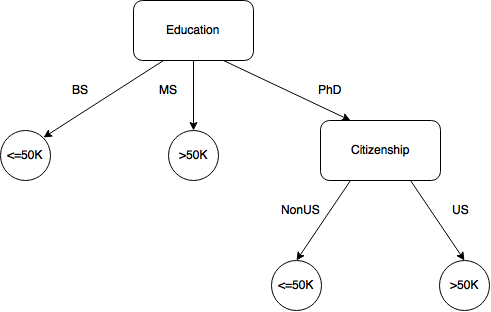
\includegraphics{dt.png}
		\item
		\begin{tabular}{| l | l | l | r |}
		\hline
		Education & Gender & Citizenship & Income \\ \hline
		PhD & male & US & $>50K$ \\ \hline
		PhD & male & nonUS & $\leq 50K$ \\ \hline
		MS & female & nonUS & $>50K$ \\ \hline
		\end{tabular}
	\end{itemize}
	\item
	\begin{itemize}
		\item
		$x = (I(Education=BS), I(Education=MS), I(Gender=male), I(Citizenship=US))$\\
		$y = 1$ if $Income \leq 50K$, $y = 0$ if $Income > 50K$\\
		So $X$, in row-based order, can be represented as following:\\
		\begin{tabular}{c | c  c  c  c}
		Observation \# & $x_{BS}$ & $x_{MS}$ & $x_{male}$ & $x_{US}$\\
		1 & 1&0&1&1\\ \hline
		2 & 0&1&1&0\\ \hline
		3 & 1&0&0&1\\ \hline
		4 & 0&0&1&0\\ \hline
		5 & 0&1&0&1\\ \hline
		6 & 0&0&0&0\\ \hline
		7 & 1&0&1&1\\ \hline
		8 & 0&0&1&1\\ \hline
		9 & 1&0&0&0\\ \hline
		10 & 0&0&0&1\\ \hline
		\end{tabular}\\
		And $Y$ is $[1,0,1,1,0,1,1,0,1,0]$
		\item
		\begin{minted}{python}
import numpy as np
from sklearn.neural_network import MLPClassifier
from sklearn.model_selection import cross_val_score
from sklearn.model_selection import KFold

trainX = [[1,0,1,1],[0,1,1,0],[1,0,0,1],[0,0,1,0],[0,1,0,1],
	[0,0,0,0],[1,0,1,1],[0,0,1,1],[1,0,0,0],[0,0,0,1]]
trainY = [1,0,1,1,0,1,1,0,1,0]
testX = [[0,0,1,1],[0,0,1,0],[0,1,0,0]]
trainX = np.asarray(trainX)
trainY = np.asarray(trainY)
testX = np.asarray(testX)

for i in range(2,6):
	kf = KFold(n_splits=5)
	total_error = 0
	for train_index, test_index in kf.split(trainX):
		clf = MLPClassifier(solver='lbfgs',hidden_layer_sizes=(i,))
		clf.fit(trainX[train_index],trainY[train_index])
		total_error += 2 - np.sum(trainY[test_index] == 
			clf.predict(trainX[test_index]))
	print("With " + str(i) + " hidden units, cross validation error is "
		+ str(total_error / 5.0))
		\end{minted}
		The cross-validated training error is shown in the following table:\\
		\begin{tabular}{c | c}
		\# of neurons & error\\
		2 & 0.6 \\
		3 & 0.4 \\
		4 & 0.2 \\
		5 & 0\\
		\end{tabular}
		\item
		The prediction is as following:\\
		\begin{tabular}{| l | l | l | r |}
		\hline
		Education & Gender & Citizenship & Income \\ \hline
		PhD & male & US & $>50K$ \\ \hline
		PhD & male & nonUS & $\leq 50K$ \\ \hline
		MS & female & nonUS & $>50K$ \\ \hline
		\end{tabular}
		The prediction is the same with the other methods.
	\end{itemize}
\end{enumerate}
\section*{Text classification}
	\subsection*{Spam classification}
		\subsubsection*{Rule-based system}
		\begin{itemize}
			\item
			dev error results of $n$ and $k$ thresholds:\\
			\begin{tabular}{l | r | r | r}
			& $k=10000$ & $k=20000$ & $k=30000$\\
			$n=1$ & 0.1059 & 0.1639 & 0.4897\\
			$n=2$ & 0.1651 & 0.1184 & 0.4779\\
			$n=3$ & 0.2044 & 0.1065 & 0.4642\\
			\end{tabular}
		\end{itemize}
		\subsubsection*{Learning to distinguish spam}
		\begin{itemize}
			\item
			Bigram features error table:\\
			\begin{tabular}{c | c | c}
			\# of examples & train error & dev error\\
			500 & 0 & 0.0910\\
			1000 & 0 & 0.0636\\
			1500 & 0 & 0.0505\\
			2000 & 0 & 0.0424\\
			2500 & 0 & 0.0380\\
			3000 & 0.0003 & 0.0380\\
			3500 & 0.0006 & 0.0349\\
			4000 & 0.0035 & 0.0312\\
			4500 & 0.0002 & 0.0324\\
			5000 & 0.0026 & 0.0368\\
			\end{tabular}\\
			Generally, the more examples for training the better accuracy will be achieved on development set. However after the number of training exceeds certain amount (4000), no additional benefit is gained through adding examples.
		\end{itemize}
	\subsection*{Sentiment classification}
	\begin{itemize}
		\item
		The error table:\\
		\begin{tabular}{l | c | c}
		& train error & dev error\\
		unigram & 0.0328 & 0.1685\\
		bigram & 0 & 0.1629
		\end{tabular}
		\item
		The error table:\\
		\begin{tabular}{c | c | c}
		\# of iterations & train error & dev error\\
		1 & 0.2920 & 0.3652\\
		2 & 0.4538 & 0.4831\\
		3 & 0.1423 & 0.2921\\
		4 & 0.5024 & 0.5112\\
		5 & 0.0499 & 0.1629\\
		6 & 0.4793 & 0.5056\\
		7 & 0.1509 & 0.3708\\
		8 & 0.0195 & 0.1629\\
		9 & 0.0292 & 0.1573\\
		10 & 0.0146 & 0.1461\\
		11 & 0.1046 & 0.3090\\
		12 & 0.0085 & 0.1685\\
		13 & 0.0389 & 0.2528\\
		14 & 0.0170 & 0.1966\\
		15 & 0.0085 & 0.1798\\
		16 & 0.0049 & 0.1798\\
		17 & 0 & 0.1629\\
		18 & 0 & 0.1629\\
		19 & 0 & 0.1629\\
		20 & 0 & 0.1629\\
		\end{tabular}\\
		The dev set error does not monotonically decrease with iteration number.\\
		This is because during the process of convergence the perceptron temporarily overfitted on (biased by) a subset of the training data that are not representative of the population, resulting in a temporary huge drop in accuracy.
	\end{itemize}
	\subsection*{Document categorization}
	\begin{itemize}
		\item
		The error table:\\
		\begin{tabular}{c | c | c}
		& train error & dev error\\
		unigram & 0.0039 & 0.1196\\
		bigram & 0 & 0.1003\\
		\end{tabular}
	\end{itemize}
\section*{Image classification}
\section*{Relating Naive Bayes classifiers and perceptrons}
First, for naive Bayes classifier we have $P(y = +1|f) \sim P(y=+1)\prod_iP(f_i|y=+1)$ and $P(y = -1|f) \sim P(y=-1)\prod_iP(f_i|y=-1)$. Since naive Bayes will classify $y$ as $+1$ when $P(y = +1|f) > P(y = -1|f)$ and vice versa, some perceptron will always classify $y$'s same as the Bayes as long as $w^Tf = P(y = +1|f) - P(y = -1|f)$.\\
We can first get the intercept $w_0$ by setting all $f_i = 0$, which means $w^Tf = w_0$, so we get:\\
\begin{eqnarray*}
w_0 &=& P(y=+1)\prod_iP(f_i=0|y=+1) - P(y=-1)\prod_iP(f_i=0|y=-1)
\end{eqnarray*}
Similarly, we can get any weight $w_j$ by setting all $f_i = 0$ except $f_j$, which means $w^Tf = w_0+w_j$, so we get:\\
\begin{eqnarray*}
w_j &=& \frac{P(y=+1)P(f_j=1|y=+1)\prod_iP(f_i=0|y=+1)}{P(f_j=0|y=+1)}\\
	&&-\frac{P(y=-1)P(f_j=1|y=-1)\prod_iP(f_i=0|y=-1)}{P(f_j=0|y=-1)}-w_0\\
	&=& \frac{P(y=+1)[P(f_j=1|y=+1)-P(f_j=0|y=+1)]\prod_iP(f_i=0|y=+1)}{P(f_j=0|y=+1)}\\
	&&-\frac{P(y=-1)[P(f_j=1|y=-1)-P(f_j=0|y=-1)]\prod_iP(f_i=0|y=-1)}{P(f_j=0|y=-1)}
\end{eqnarray*}
Since all the probabilities are non-zero, we have proven that such binary naive Bayes can be represented by a perceptron that always produces the same decision.
\end{onehalfspace}
\end{document}